\chapter{Containerized Applications}\label{containerized-applications}

This chapter introduces containers' core concepts, differences from
previous virtualization and container technologies, and how the use case
application could be containerized.

\section{Container Runtime}\label{container-runtime}

\emph{Docker Engine} was released at the beginning of 2013 from a PaaS
company, as a lightweight alternative to VMs to running and develop
components of applications. Since then, it gained consent by large part
of IT industry and today it's the de-facto standard for container
technologies.

While traditional container technologies like OpenVZ aimed to emulate a
full functional operating system, Docker focused only on running single
processes, separating the application from the OS.

Some of the advantages in using Docker are:

\begin{itemize}
\itemsep1pt\parskip0pt\parsep0pt
\item
  reproducible and standardized environments between development,
  staging, QA and production
\item
  reduce overhead respect to VMs used for deploy single application
\item
  improve isolation and security respect to OS that hosts more
  applications
\end{itemize}

Under the hood, Docker Engine it's composed mainly by a Git-like command
line interface, a daemon and \emph{libcontainer}, a library that use
Linux kernel capabilities such as \emph{namespaces} and \emph{cgroups}.

\begin{figure}[htbp]
\centering
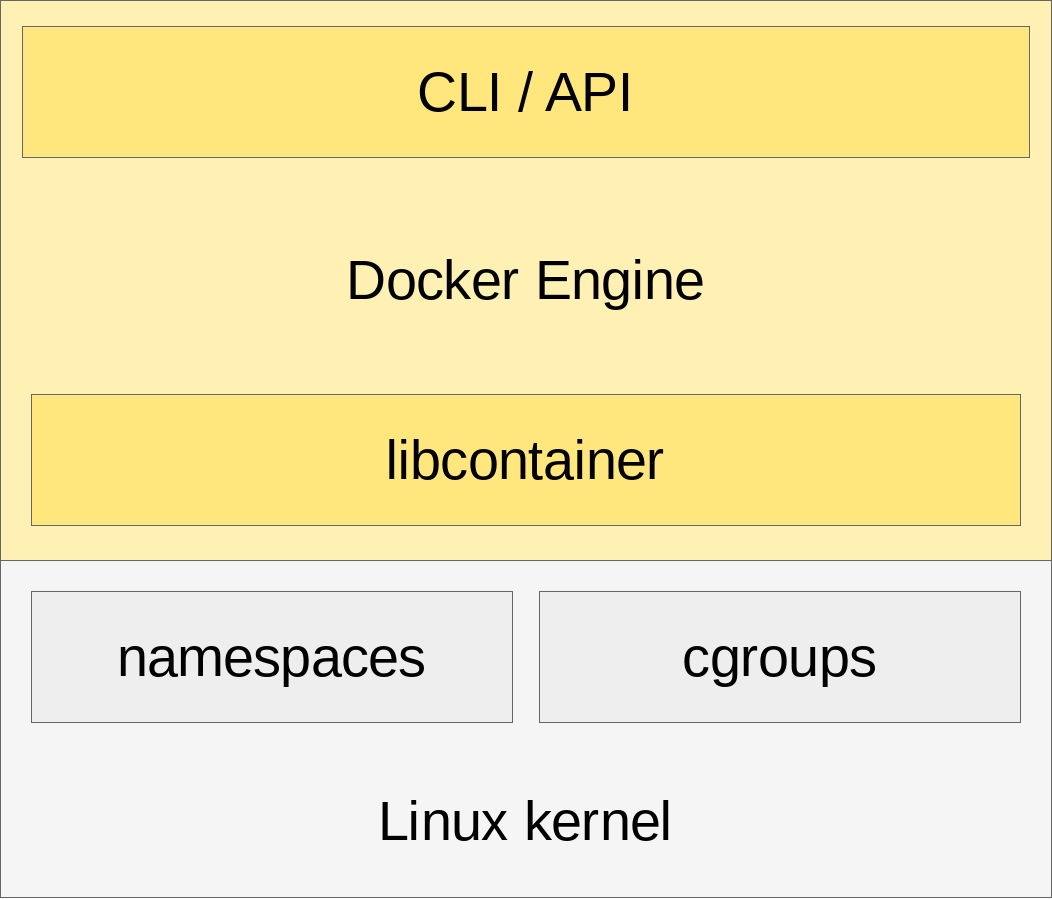
\includegraphics{media/ch3-docker.png}
\caption{Overview of Docker Engine}
\end{figure}

\begin{figure}[htbp]
\centering
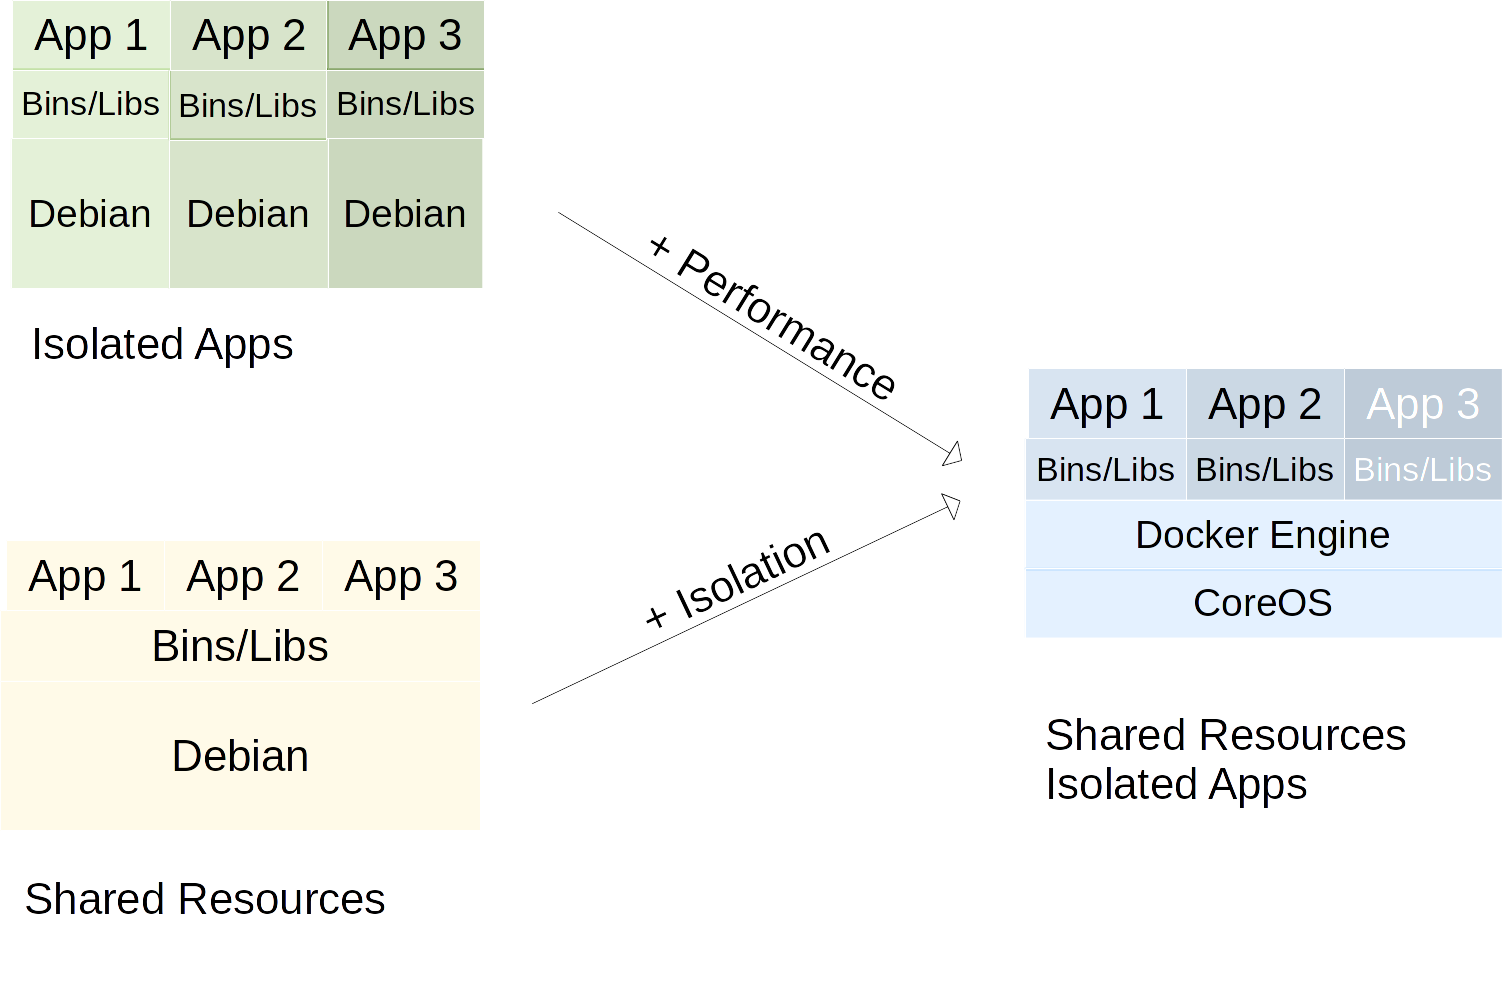
\includegraphics{media/ch3-docker_multiapps.png}
\caption{Performance and Isolation in Multiapps Deployment}
\end{figure}

Someone sees containers more as ``lightweight VMs'', so has been
prepared an alternative base image
(https://github.com/phusion/baseimage-docker). In this case there are a
canonical init daemon as PID 0, instead of the application process
itself. This was particular useful in the early period since it was
needed for some components that depends on specific system feature, such
as syslog, and other purposes. But today Docker includes directly that
kind of features, so this need is decreased.

\begin{itemize}
\itemsep1pt\parskip0pt\parsep0pt
\item
  Part 1
  (http://blog.phusion.nl/2015/01/20/docker-and-the-pid-1-zombie-reaping-problem/)
\item
  Part 2
  (http://blog.phusion.nl/2015/01/20/baseimage-docker-fat-containers-treating-containers-vms/)
\end{itemize}

There are also alternative container runtimes, such as \emph{rkt} (read
``rocket'') (https://github.com/coreos/rocket) that focuses on
reliability and security in production environment.

On June 22, 2015 was announced the \emph{Open Container
Project}\cite{OpenContainerProject} from \emph{Linux Foundation} and
major companies with the target of an industry-wide standard, taking
Docker as the starting point.

\section{Gasista Felice's
Architecture}\label{gasista-felices-architecture}

To apply this to the use case Gasista Felice, the first step is
splitting the application in well-defined components, then containerize
one by one.

In a traditional way, one would have said that the components are
AngularJS for frontend, and Django and PostgreSQL for backend. Instead,
in DevOps-oriented context with dev/prod parity, components should be
the same used in production:

\begin{itemize}
\itemsep1pt\parskip0pt\parsep0pt
\item
  \emph{NGiNX}, web/caching server and reverse proxy
\item
  \emph{harp}, frontend server with built-in preprocessors
\item
  \emph{uWSGI}, web application server
\item
  \emph{PostgreSQL}, relational database
\end{itemize}

In addition, following che \emph{12factor} guidelines, a convention is
to use:

\begin{itemize}
\itemsep1pt\parskip0pt\parsep0pt
\item
  environment variables for configuration
\item
  TCP sockets for inter-container communication
\end{itemize}

So Django settings should be based on \emph{environment variables} with
some defaults. Has been chosen \texttt{APP\_ENV} as main variable that
determines a different behavior of backend. For example, when in
development environment, there is the need of reloading app as soon as
possible with code changes, while in production environment there will
need of more workers and a periodical offloading task.

Another convention is to minimize the mutating components, so the file
system should be read-only by default (including binaries and
libraries), and only well defined directories should be writable
(e.g.~files uploaded by application users).

\section{Container Images}\label{container-images}

As of virtual machines consists of a base disk image and one or more
instances, so containers providers base images and one or more instances
(``real'' containers) running on. In particular, Docker applies the
concept of \emph{Copy on Write} (CoW) that consist of, starting from a
well-defined file system status, write only the differences from it, in
order to minimize the disk usage.

There are base images of common operating system (Debian, Ubuntu,
CentOS) but also language-specific runtimes (Python, NodeJS, Java).
Starting from here it's possible build custom images contains the
application components. In addition, every image has one or more
\emph{tags} in order to provide different versions: e.g.~in
\texttt{debian:8} the \texttt{8} is the tags part that identifies
\emph{Debian Jessie}, but it's also possible define the Debian testing
image with \texttt{debian:9}.

The main way to build Docker images is via \emph{Dockerfiles}, files
that include:

\begin{itemize}
\itemsep1pt\parskip0pt\parsep0pt
\item
  the base image via the \texttt{FROM} directive
\item
  a \texttt{MAINTAINER} reference
\item
  \texttt{ENV}ironment variables declaration
\item
  \texttt{COPY}ing data inside the image
\item
  \texttt{RUN} commands
\item
  TCP ports to expose via \texttt{EXPOSE} directive
\item
  \texttt{CMD} as the default command to run when starting the container
\item
  others as defined in Docker builder reference
  (https://docs.docker.com/reference/builder/)
\end{itemize}

Following the Docker best practices
(https://docs.docker.com/articles/dockerfile\_best-practices/) has been
developed some images as shown in the following picture:

\begin{figure}[htbp]
\centering
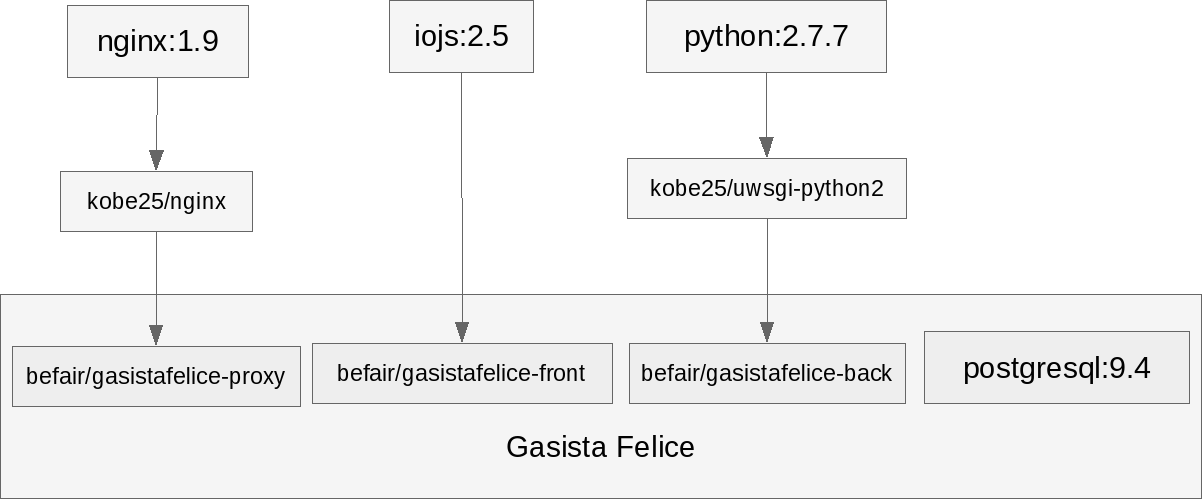
\includegraphics{media/ch3-images_tree.png}
\caption{Container Images Dependency Tree}
\end{figure}

In order to follow the DRY principle, has been developed \texttt{nginx}
and \texttt{uwsgi-python2} base images that provides a common
environment for potential other containerized applications.

The backend of Gasista Felice is an application written in Python with
Django web framework, and served by uWSGI application server. In the
base image has been setted default values for uWSGI, Python, Debian and
PostgreSQL client, were added an \emph{app} Unix user/group and were
installed uWSGI and Python core packages. Note that since uWSGI is the
default process, when a real container will be started, uWSGI take all
the configuration from these defaults and eventual future additions of
overriding.

Then the Dockerfile of Gasista Felice backend, including installation of
dependencies, and copying of application code.

The NGiNX/proxy component also has a base image that move logging to
stdout/stderr and other small customizations.

Instead the Gasista Felice proxy Dockerfile provide a production-ready
configuration, with static files caching.

Another components consist of the Harp server that served static
processed content of frontend. In future this component could be
eliminated, since once the files are generated they could be served
directly from NGiNX.

The PostgreSQL image instead is ready as it is, so it's not be
customized.

\section{Container Orchestration}\label{container-orchestration}

Since an application is splitted in more well-defined components, there
is also the need of a container orchestrator in order to run a multi-container application.

For this target has been chosen \emph{Docker Compose}
(https://docs.docker.com/compose/), a basic tool to deploy applications
in development, similar to Vagrant for VMs. Docker Compose will resolve
the dependency graph of components and linked them together. While
Docker Engine provides the core capabilities, Docker Compose represent
the tool developers use the majority of time.

Following the \href{https://docs.docker.com/compose/yml/}{docker-compose.yml reference}, the containers was orchestrated
(only for development) with \emph{Docker Compose}. So running the whole
application is simple as run \texttt{docker-compose\ up} command!

\begin{figure}[htbp]
\centering
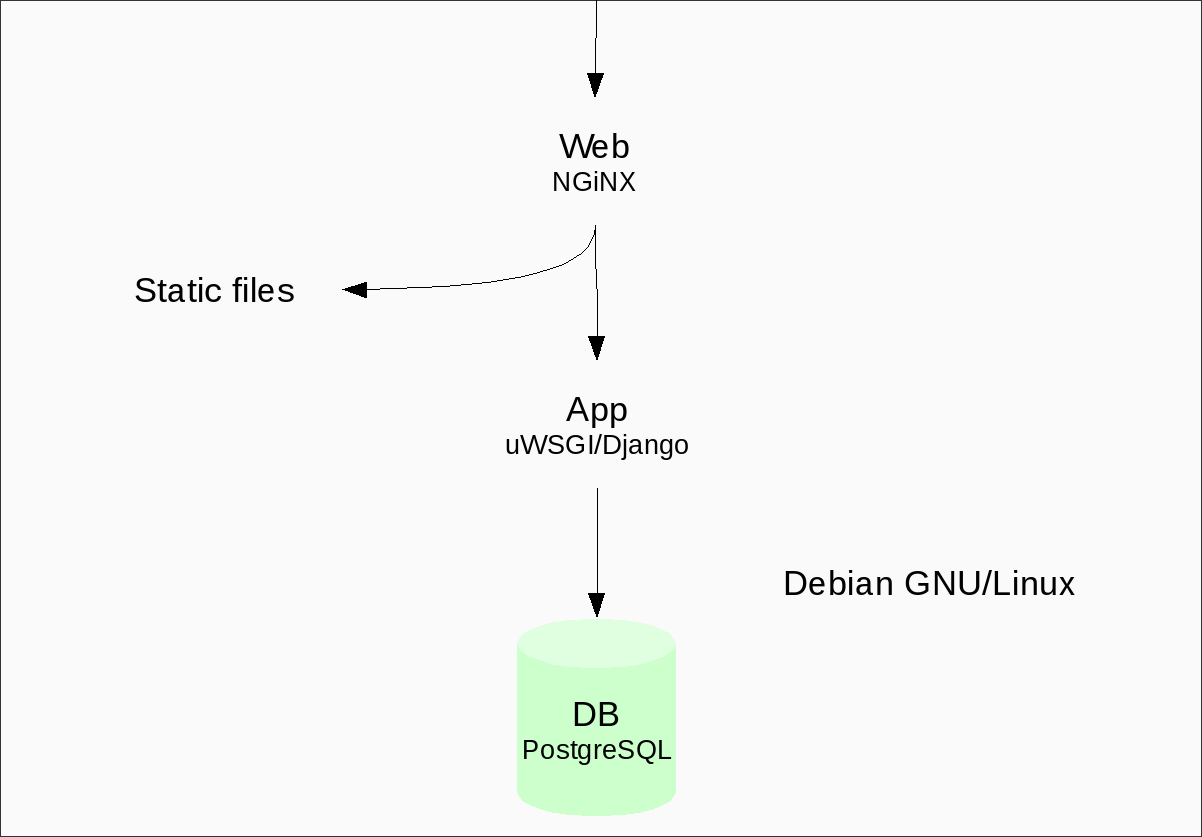
\includegraphics{media/ch3-gf_old.png}
\caption{Gasista Felice before containerization}
\end{figure}

\begin{figure}[htbp]
\centering
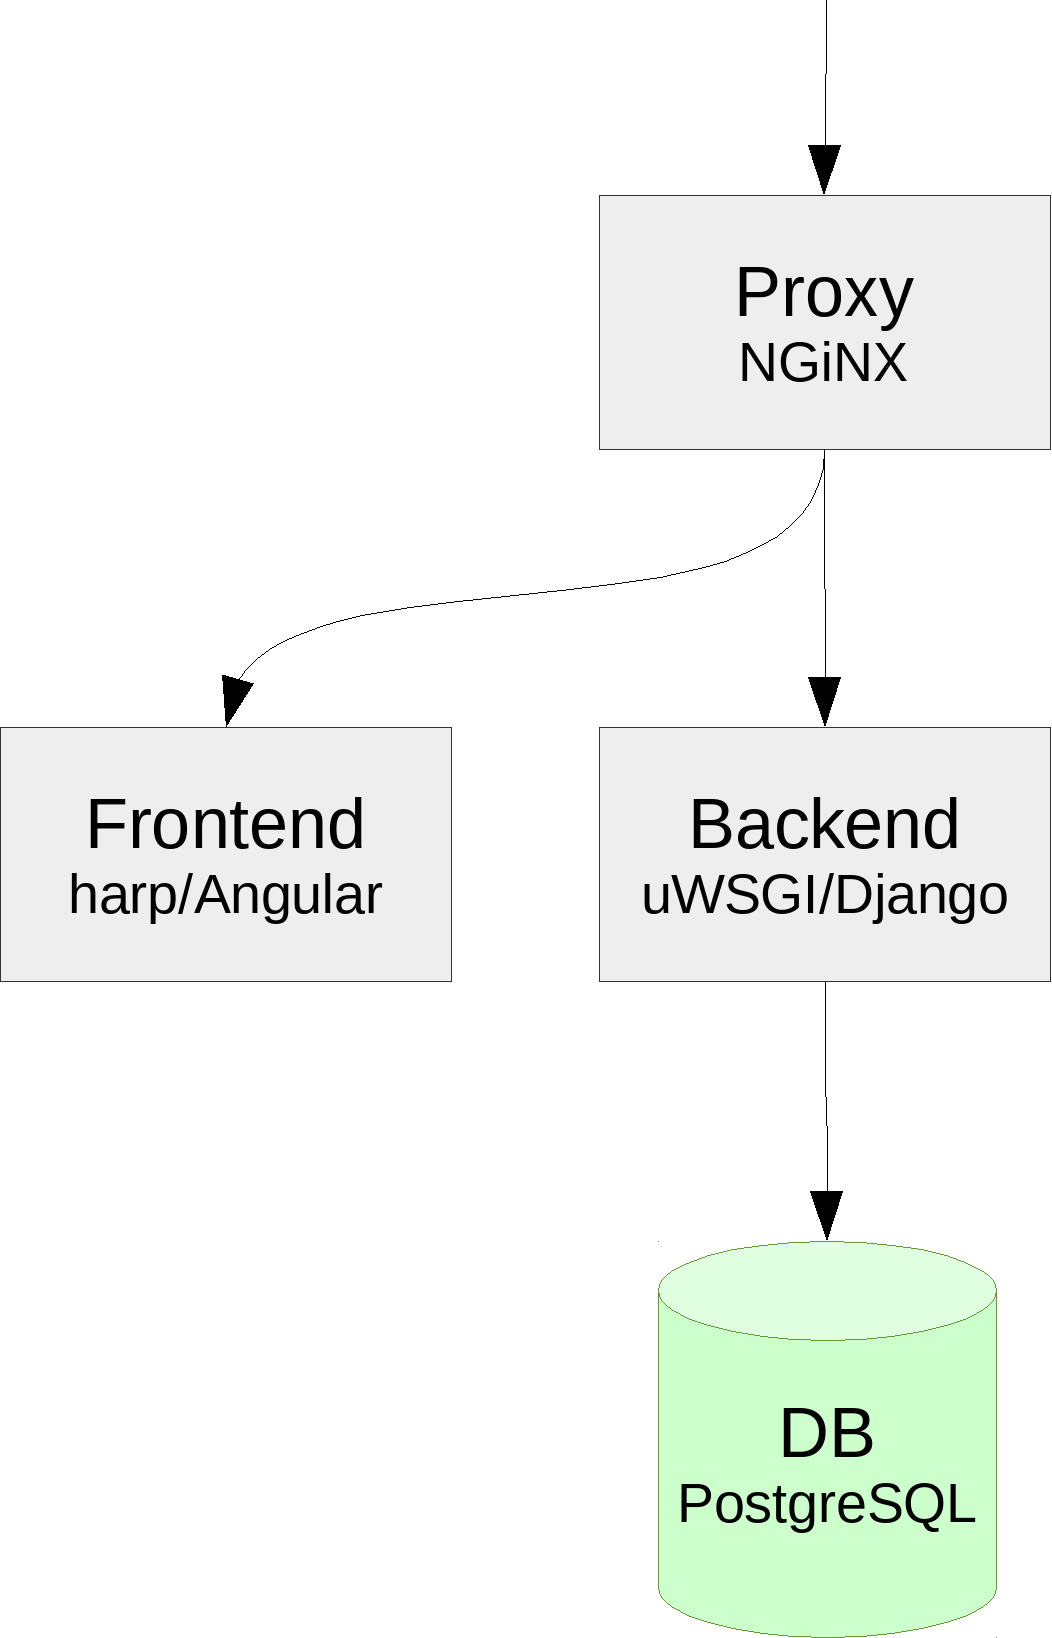
\includegraphics{media/ch3-gf.png}
\caption{Gasista Felice after containerization}
\end{figure}